\documentclass[12pt]{article}
\usepackage[utf8]{inputenc}
\usepackage[english]{babel}
\usepackage{amsfonts}
\usepackage{amssymb}
\usepackage{graphicx}
\newlength\tindent
\setlength{\tindent}{\parindent}
\setlength{\parindent}{0pt}
\renewcommand{\indent}{\hspace*{\tindent}}
\usepackage[margin=0.5in]{geometry}
\usepackage{listings}
\usepackage{enumerate}


\begin{document}

\begin{titlepage}
\begin {center}
\Huge Bluetooth Racer\\


\Large Erik Sargent\\
\Large Weston Jensen\\
\Large David Christensen\\
December 2015\\
\end {center}

\end{titlepage}


\tableofcontents
\newpage

\section{Design Documentation}

 

\section{Introduction}

This document describes the design and process of changing a remote control car into a Bluetooth controlled racer. A simple App was developed so that the movement of a smartphone controls the acceleration and steering of the car. The object is to enable the car to turn left and right, and move forward and backward, all controlled by the Bluetooth connection to the phone.\\

\section{Scope}
This document discusses, in detail, the electrical and software design for the Bluetooth Racer. It includes the requirements, dependencies and theory of operation. Schematics and code segments are used to give a more thorough explanation of the design. Testing procedures and results of each requirement are included. The complete code is located in Appendix B.\\

\section{Design Overview}
\subsection{Requirements}
The following are the given requirements for Bluetooth Racer:\\
1. The system shall use the Tiva C Series TM4C123GH6PM microcontroller.\\
2. The system shall use two external batteries. A 5 volt battery with USB connection to the microcontroller and a 9 volt DC supply for the drive and steering.\\
3. The system shall use a Bluetooth 4.0 Module.\\
4. The system shall use a Dual TB6612FNG Motor Driver (H-Bridge).\\
5. The Racer shall have PWM output to controller variable motor speed.\\
6. Working LED’s should be used for the front and tail lights, as well as an inside light.\\
7. Upon powering up, the inside light should be turned on. \\
8. Upon connecting to Bluetooth, the front and tail lights should turn on. \\
9. The microcontroller will transmit and receive data from the Bluetooth module through UART.\\
10. The user shall command the Racer with a smartphone over Bluetooth connection. The movement of the phone will control the direction in which the car will move.\\
11. The Racer shall be able to turn and drive forward and backward on command of the user.\\


\subsection{Materials}
The following are dependencies for the Bluetooth Racer:\\
\begin{enumerate}
\item An RC car with working motors for both steering and driving.
\item A 9 volt DC power supply
\item A 5 volt DC power supply with USB connection
\item Dual TB6612FNG Motor Driver
\item Tiva C Series TM4C123GH6PM microcontroller
\item Bluetooth 4.0 Module
\item Schmidt Trigger
\item 5 LEDs
\item Spray Paint
\item NPN Transistor
\item Assorted resistors and capacitors
\end{enumerate}

\section{Testing}
As specified before, the car is controlled via Bluetooth. The iOS app sends a 1 byte command that the UART module on the micro-controller receives. This byte of data contains the information necessary to enable the two H-bridges and the data to set the variable speed for PWM. The byte of data is represented in the following format: two bits for H-bridge drive followed by two bits to set the variable speed, these four bits are followed by two bits for H-bridge turn followed by two bits to set the variable speed\\

\begin {center}
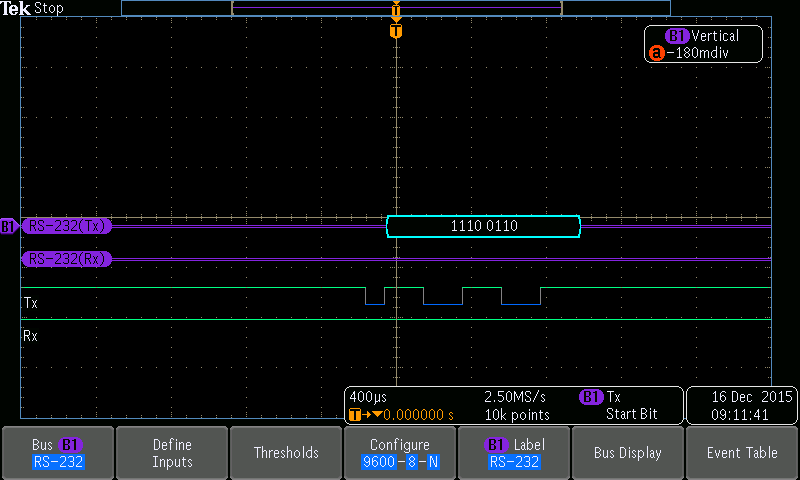
\includegraphics[scale=.75]{uart-message}
\\
Figure 1	
\end {center}



\begin {center}
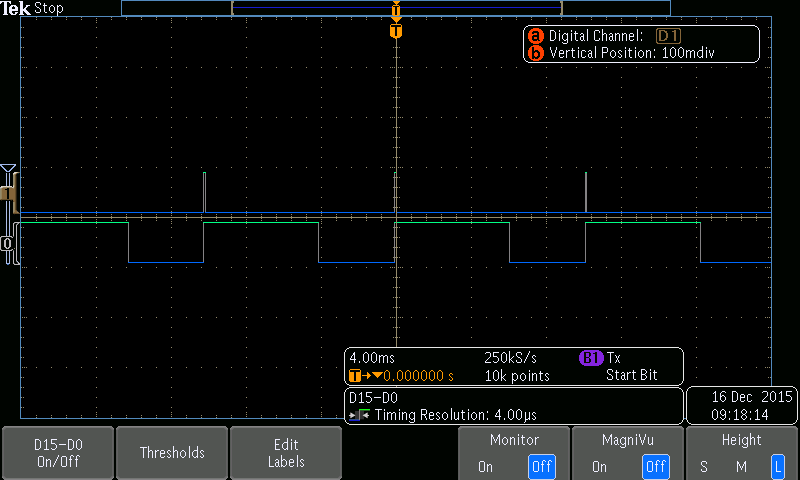
\includegraphics[scale=.75]{half-power}
\\
Figure 2
\end {center}
\begin {center}
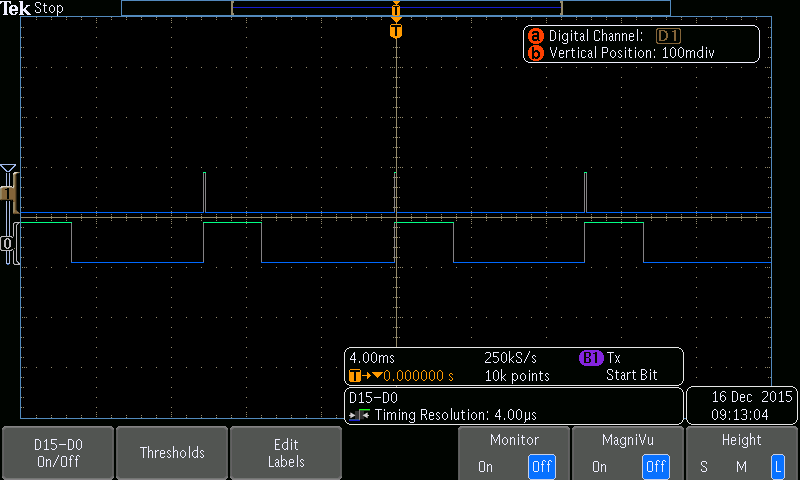
\includegraphics[scale=.75]{quarter-power}
\\
Figure 3
\end {center}

\end{document}